\documentclass[12pt,a4paper]{report}
% ---------------- Packages ----------------
\usepackage[T1]{fontenc}
\usepackage{mathptmx}          % Times-style font, common college requirement
\usepackage{xcolor}
\usepackage{graphicx}
\usepackage{geometry}
\usepackage{setspace}
\usepackage{enumitem}
\usepackage{needspace}
\usepackage{pdfpages}
\usepackage{titlesec}
\usepackage{fancyhdr}
\usepackage{tocloft}
\usepackage{amsmath}
\usepackage{amssymb}
\usepackage{listings}
\usepackage{booktabs}
\usepackage{longtable}
\usepackage{array}
\usepackage{float}
\usepackage{caption}
\usepackage{xurl}
\usepackage{tikz}
\usetikzlibrary{arrows.meta,positioning,shapes.multipart}

% ---------------- Version macros ----------------
% EDIT these three lines to match composer.json / package.json
\newcommand{\LV}{Laravel~13}
\newcommand{\TW}{Tailwind~CSS~4}
\newcommand{\VITE}{Vite~8}

% ---------------- List of Figures / Tables (no dotted leaders) ----------------
\renewcommand{\cftfigpresnum}{Figure }
\renewcommand{\cftfigaftersnum}{}
\setlength{\cftfigindent}{0pt}
\setlength{\cftfignumwidth}{1.25in}
\renewcommand{\cftfigleader}{\hfill}
\setlength{\cftbeforefigskip}{12pt}
\renewcommand{\cftfigfont}{\normalfont}
\renewcommand{\cftfigpagefont}{\normalfont}

\renewcommand{\cfttabpresnum}{Table }
\renewcommand{\cfttabaftersnum}{}
\setlength{\cfttabindent}{0pt}
\setlength{\cfttabnumwidth}{1.25in}
\renewcommand{\cfttableader}{\hfill}
\setlength{\cftbeforetabskip}{12pt}
\renewcommand{\cfttabfont}{\normalfont}
\renewcommand{\cfttabpagefont}{\normalfont}

% ---------------- Page Setup ----------------
\geometry{left=1.25in,right=1in,top=1in,bottom=1in}
\onehalfspacing
\setlength{\emergencystretch}{3em}
\setlength{\parindent}{0pt}
\setlength{\parskip}{8pt}
\setlength{\headheight}{14pt}

% ---------------- Custom Font Commands ----------------
\newcommand{\headingSixteen}[1]{{\fontsize{16pt}{18pt}\selectfont\textbf{#1}}}
\newcommand{\headingFourteen}[1]{{\fontsize{14pt}{16pt}\selectfont\textbf{#1}}}

% ---------------- Section Formatting ----------------
% Section 15 pt, subsection 13 pt, so the hierarchy is visible
\titlespacing*{\section}{0pt}{16pt}{10pt}
\titlespacing*{\subsection}{0pt}{12pt}{6pt}
\titleformat{\section}{\bfseries\fontsize{15pt}{17pt}\selectfont}{\thesection}{0.8em}{}
\titleformat{\subsection}{\bfseries\fontsize{13pt}{15pt}\selectfont}{\thesubsection}{0.7em}{}

% ---------------- Header & Footer ----------------
\fancypagestyle{maincontent}{
\fancyhf{}
\fancyhead[R]{\small \textit{FinSight AI}}
\fancyfoot[L]{\small \textit{Saintgits College of Engineering (Autonomous)}}
\fancyfoot[R]{\small \thepage}
\renewcommand{\headrulewidth}{0pt}
\renewcommand{\footrulewidth}{0pt}
}
% Front matter: count pages internally using Roman numerals, but do not print
% page numbers on the preliminary pages, matching the supplied SIIP template.
\fancypagestyle{frontmatter}{
\fancyhf{}
\renewcommand{\headrulewidth}{0pt}
\renewcommand{\footrulewidth}{0pt}
}
% Chapter title pages: no header, no footer
\fancypagestyle{plain}{
\fancyhf{}
\renewcommand{\headrulewidth}{0pt}
\renewcommand{\footrulewidth}{0pt}
}

% ---------------- Bibliography Spacing ----------------
\makeatletter
\renewenvironment{thebibliography}[1]
{\@mkboth{}{}%
\list{\@biblabel{\@arabic\c@enumiv}}%
{\settowidth\labelwidth{\@biblabel{#1}}%
\leftmargin\labelwidth
\advance\leftmargin\labelsep
\itemsep=0.6\baselineskip
\usecounter{enumiv}%
\let\p@enumiv\@empty
\renewcommand\theenumiv{\@arabic\c@enumiv}}%
\sloppy}
{\endlist}
\makeatother

% ---------------- Helpers ----------------
\newcommand{\chrow}[3]{\textbf{CHAPTER #1} & \textbf{\MakeUppercase{#2}} & \textbf{\pageref{#3}}\\[3pt]}
\newcommand{\secrow}[3]{#1 & #2 & \pageref{#3}\\}

% College logo with fallback (file name has no spaces)
\newcommand{\collegelogo}[1]{%
\IfFileExists{Saintgits_logo.png}{\includegraphics[width=#1]{Saintgits_logo.png}}{\rule{0pt}{1.2cm}}}

% Screenshot with placeholder fallback: file, width, box height, title, description
\newcommand{\shot}[5]{%
\IfFileExists{#1}{\includegraphics[width=#2\textwidth]{#1}}{%
\fbox{\parbox[c][#3][c]{0.85\textwidth}{\centering\textbf{#4}\\[0.2cm]\small #5\\[0.2cm]\textit{Upload \texttt{\detokenize{#1}} to Overleaf}}}}}

\lstdefinelanguage{PHP}{
  keywords={abstract, and, array, as, bool, boolean, break, case, catch, class, clone, const, continue, declare, default, die, do, echo, else, elseif, empty, enddeclare, endfor, endforeach, endif, endswitch, endwhile, eval, exit, extends, false, final, finally, float, for, foreach, function, global, goto, if, implements, include, include_once, instanceof, insteadof, int, integer, interface, isset, list, match, namespace, new, null, or, print, private, protected, public, readonly, require, require_once, return, static, string, switch, throw, trait, true, try, unset, use, var, while, xor, yield},
  sensitive=true,
  morecomment=[l]{//},
  morecomment=[l]{\#},
  morecomment=[s]{/*}{*/},
  morestring=[b]',
  morestring=[b]"
}
\lstset{
  basicstyle=\ttfamily\footnotesize,
  frame=single,
  rulecolor=\color{gray!40},
  backgroundcolor=\color{gray!5},
  numbers=none,
  columns=flexible,
  keepspaces=true,
  breaklines=true,
  showstringspaces=false,
  xleftmargin=6pt,
  xrightmargin=6pt,
  aboveskip=10pt,
  belowskip=10pt
}

% Numbered chapters: centered chapter opener on its own page, as in the template
\titleformat{\chapter}[display]
{\centering\fontsize{16pt}{18pt}\selectfont\bfseries}
{\vspace*{\fill}CHAPTER \thechapter}{10pt}
{\MakeUppercase}
[\label{chaptertitle-\thechapter}\vspace*{\fill}\clearpage]
\titlespacing*{\chapter}{0pt}{0pt}{0pt}
\titleformat{name=\chapter,numberless}[display]
{\centering\fontsize{16pt}{18pt}\selectfont\bfseries}
{}{0pt}
{\vspace*{\fill}\MakeUppercase}
[\vspace*{\fill}\clearpage]

\captionsetup[figure]{name=Figure, labelsep=colon}
\captionsetup[table]{labelsep=colon}
\usepackage[hidelinks]{hyperref}

\begin{document}
\pagenumbering{roman}

% ===================== TITLE PAGE =====================
\thispagestyle{empty}
\begin{center}
\vspace*{0.3cm}
\headingSixteen{SUMMER INDUSTRY IMMERSION PROGRAMME}\\[0.25cm]
\headingFourteen{ON}\\[0.25cm]
\headingSixteen{FINSIGHT AI: INTELLIGENT PERSONAL FINANCE \& PREDICTIVE ANALYTICS PLATFORM}\\[0.6cm]
\headingFourteen{Submitted By}\\[0.15cm]
\headingFourteen{SHIJO VARGHESE - MGP25MCA-2055}\\[0.6cm]
\headingFourteen{To}\\[0.15cm]
\textit{the APJ Abdul Kalam Technological University in partial}\\
\textit{fulfillment of the requirements for the award of the degree of}\\[0.4cm]
\headingFourteen{MASTER OF COMPUTER APPLICATIONS}\\[0.6cm]
\headingFourteen{Under the guidance of}\\[0.2cm]
\headingFourteen{Mr. Jacob Zachariah}\\
\headingFourteen{Assistant Professor}\\[0.8cm]
\collegelogo{3.8cm}\\[0.8cm]
\headingFourteen{DEPARTMENT OF COMPUTER APPLICATIONS}\\[0.15cm]
\headingFourteen{SAINTGITS COLLEGE OF ENGINEERING (AUTONOMOUS)}\\
\headingFourteen{PATHAMUTTOM, KOTTAYAM, KERALA -- 686532}\\[0.25cm]
\textit{(Approved by AICTE and affiliated to APJ Abdul Kalam Technological University)}\\[0.5cm]
\headingSixteen{JULY 2026}
\end{center}

% ===================== BONAFIDE =====================
\newpage
\thispagestyle{empty}
\begin{center}
\fontsize{16pt}{18pt}\selectfont
\textbf{SAINTGITS COLLEGE OF ENGINEERING (AUTONOMOUS)}\\
Kottukulam Hills, Pathamuttom, Kottayam, Kerala -- 686532
\end{center}
\vspace{0.2cm}
\begin{center}\collegelogo{4.5cm}\end{center}
\vspace{0.1cm}
\begin{center}\fontsize{16pt}{18pt}\selectfont\textbf{BONAFIDE CERTIFICATE}\end{center}
\vspace{0.2cm}

Certified that the report entitled \textbf{``FinSight AI: Intelligent Personal Finance \& Predictive Analytics Platform''} submitted by \textbf{``SHIJO VARGHESE - MGP25MCA-2055''} to the APJ Abdul Kalam Technological University in partial fulfillment of the requirements for the award of the Degree of \textbf{Master of Computer Applications} is a bonafide record of the \textbf{Summer Industry Immersion Programme (SIIP)} work carried out by him under our guidance and supervision. This report in any form has not been submitted to any other University or Institute for any purpose.

\vspace{2.2cm}
\noindent
\begin{minipage}[t]{0.45\textwidth}
\raggedright\textbf{Mr. Jacob Zachariah}\\Internal Guide
\end{minipage}
\hfill
\begin{minipage}[t]{0.45\textwidth}
\raggedleft\textbf{Ms. Ankitha Philip}\\SIIP Coordinator
\end{minipage}

\vspace{1.5cm}
\begin{center}
\begin{minipage}{0.45\textwidth}
\centering\textbf{Dr. Rani Saritha R}\\Head of the Department
\end{minipage}
\end{center}

\vspace{1.5cm}
\noindent
\begin{minipage}[t]{0.45\textwidth}\raggedright Internal Examiner\end{minipage}
\hfill
\begin{minipage}[t]{0.45\textwidth}\raggedleft External Examiner\end{minipage}

% ===================== ORGANIZATION CERTIFICATE =====================
\newpage
\thispagestyle{empty}
\begin{center}
\fontsize{16pt}{18pt}\selectfont
\textbf{Certificate from the Organization}
\end{center}
\vspace{0.5cm}
\begin{center}
\IfFileExists{Internship_Certificate_Updated.pdf}{
\includegraphics[page=1,width=\textwidth,height=0.88\textheight,keepaspectratio]{Internship_Certificate_Updated.pdf}
}{
\fbox{\parbox[c][12cm][c]{0.85\textwidth}{
\centering \textbf{[ CodeDesign Technologies Internship Certificate Placeholder ]}\\
\vspace{0.5cm}
\textit{Upload Internship\_Certificate\_Updated.pdf to Overleaf}
}}
}
\end{center}

% ===================== ACKNOWLEDGEMENT =====================
\clearpage
\pagestyle{frontmatter}
\begin{center}
\fontsize{16pt}{18pt}\selectfont
\textbf{ACKNOWLEDGEMENT}
\end{center}
\vspace{1cm}

At the outset, I thank the Almighty God for His abundant grace, wisdom, strength and blessing to make this endeavour a success. I express my sincere gratitude to \textbf{Dr. Sudha T.}, Principal, Saintgits College of Engineering (Autonomous), for her warm encouragement and to the college management for providing high-quality infrastructural and computing facilities.

I place on record my heartfelt gratitude to \textbf{Prof. Mini Punnoose}, Director, Department of Computer Applications, for her constant motivation and valuable advice. I also convey my earnest gratitude to \textbf{Dr. Rani Saritha R}, Head of the Department, Department of Computer Applications, for her consistent support and constructive guidance throughout the programme.

I express my deepest gratitude to my SIIP internal guide, \textbf{Mr. Jacob Zachariah}, Assistant Professor, and to \textbf{Ms. Ankitha Philip}, the SIIP Coordinator, for their continuous mentorship, perceptive suggestions, regular assessments and encouragement during the course of this project.

I am indebted to the management of \textbf{CodeDesign Technologies Pvt. Ltd}, Kochi, for giving me the opportunity to undertake my 45-day internship in Website Development. I am thankful to the mentors and engineers of the team for their guidance, for the feedback they gave on my work and for introducing me to professional web development practice.

Finally, I thank my parents and friends for their patience, moral support and steadfast encouragement throughout my academic studies and this project.

\vspace{2cm}
\begin{flushright}\textbf{Shijo Varghese}\end{flushright}

% ===================== ABSTRACT =====================
\clearpage
\begin{center}
\fontsize{16pt}{18pt}\selectfont
\textbf{ABSTRACT}
\end{center}
\vspace{0.6cm}

\noindent
This report documents the work carried out during a 45-day internship in Website Development (16 May to 30 June 2026) under the Summer Industry Immersion Programme (SIIP) at CodeDesign Technologies Pvt. Ltd, Kochi, where \textbf{FinSight AI}, a full-stack personal finance, financial physics, and predictive analytics platform, was designed and built. Conventional finance applications act as passive ledgers: they demand manual data entry, give generic advice, and offer little forward-looking insight or behavioral friction. FinSight AI addresses these gaps by combining modern web engineering with real-time financial physics, multi-perspective AI deliberation, statistical forecasting, and conversational intelligence.

\par\vspace{6pt}
\noindent
The platform is built with \textbf{\LV{}} (PHP 8.3) in an MVC architecture, \textbf{SQLite} for persistence, and \textbf{\TW{}}, \textbf{Alpine.js} and \textbf{Chart.js} on the front end. It supports multi-source income tracking, categorised expenses, category budgets with threshold alerts, goal tracking and investment monitoring. Advanced analytical and behavioral modules include a 60 FPS sub-paise \textbf{Financial Independence Telemetry Engine} ($V = C - B$), an Autonomous AI \textbf{Capital Council} for multi-perspective purchase audits, a 4-D \textbf{Capital Allocation Radar}, an Automated \textbf{Overnight Cash Sweep}, a least-squares linear regression cash flow forecaster, a ``Time Machine'' loan commitment simulator, a \textbf{Financial Multiverse} for branching timelines (``Git for money''), an \textbf{Impulse Shield} with a 48-hour temptation vault, a heuristic \textbf{FinScore} (0--1000) health indicator, a Hidden Subscription Hunter, a Section 80C tax tracker, a UPI SMS auto-parser, and rental-property benchmarking.

\par\vspace{6pt}
\noindent
The AI layer integrates \textbf{Google Gemini 2.5 Flash} for a context-aware conversational advisor with conversational memory, dual-persona modes (Professional and Roast), an interactive voice CFO (JARVIS), and a resilient 15-topic local fallback engine. The report describes the design, implementation, testing of 57 automated test suites, limitations and learning outcomes of the project.

\par\vspace{10pt}
\noindent
\textbf{Keywords:} personal finance, Laravel, large language model, Gemini, linear regression, predictive analytics, financial physics, FinScore, financial multiverse.

% ==========================================================
% TABLE OF CONTENTS (single page, manual)
% ==========================================================
\clearpage
\begin{center}
{\fontsize{16pt}{18pt}\selectfont\textbf{TABLE OF CONTENTS}}
\end{center}
\vspace{0.25cm}
\begingroup
\renewcommand{\arraystretch}{0.95}
\setlength{\tabcolsep}{3pt}
\setlength{\LTpre}{0pt}
\setlength{\LTpost}{0pt}
\setlength{\parskip}{0pt}
\fontsize{10pt}{11.5pt}\selectfont
\newcommand{\tocsub}[1]{\hspace*{0.25cm}#1}

\begin{longtable}{
>{\raggedright\arraybackslash}p{1.0in}
>{\raggedright\arraybackslash}p{3.85in}
>{\centering\arraybackslash}p{0.85in}
}
\textbf{CHAPTER} & \centering\textbf{TITLE} & \textbf{PAGE NO.} \tabularnewline
\textbf{CHAPTER 1} & \textbf{INTRODUCTION} & \pageref{chaptertitle-1} \\
1.1 & About the Summer Industry Immersion Programme & \pageref{s11} \\
1.2 & Objectives of the Internship & \pageref{s12} \\
1.3 & Scope of the Internship & \pageref{s13} \\
\textbf{CHAPTER 2} & \textbf{ORGANIZATION PROFILE} & \pageref{chaptertitle-2} \\
2.1 & Introduction to the Organization & \pageref{s21} \\
\tocsub{2.1.1} & \tocsub{Location and Reach} & \pageref{s211} \\
2.2 & Philosophy and Approach & \pageref{s22} \\
\tocsub{2.2.1} & \tocsub{What Sets the Company Apart} & \pageref{s221} \\
2.3 & Services Offered & \pageref{s23} \\
\textbf{CHAPTER 3} & \textbf{INTERNSHIP WORK} & \pageref{chaptertitle-3} \\
3.1 & Internship Objectives & \pageref{s31} \\
3.2 & Technologies and Tools Used & \pageref{s32} \\
3.3 & Hardware and Software Requirements & \pageref{s33} \\
3.4 & Tasks and Responsibilities Assigned & \pageref{s34} \\
3.5 & Weekly Assigned Tasks & \pageref{s35} \\
\textbf{CHAPTER 4} & \textbf{WORK CARRIED OUT} & \pageref{chaptertitle-4} \\
4.1 & Project Overview & \pageref{s41} \\
4.2 & System Design & \pageref{s42} \\
\tocsub{4.2.1} & \tocsub{Architectural Framework \& Layered Design} & \pageref{s421} \\
\tocsub{4.2.2} & \tocsub{Mathematical Formulations} & \pageref{s422} \\
\tocsub{4.2.3} & \tocsub{Worked Example: Regression Forecast} & \pageref{s4221} \\
\tocsub{4.2.4} & \tocsub{Database Design} & \pageref{s4222} \\
\tocsub{4.2.5} & \tocsub{Use Case Diagram} & \pageref{s423} \\
\tocsub{4.2.6} & \tocsub{Activity Diagram} & \pageref{s424} \\
4.3 & Modules or Functional Description & \pageref{s43} \\
4.4 & Implementation Performed & \pageref{s44} \\
4.5 & Testing and Validation & \pageref{s441} \\
4.6 & Screenshots of Work & \pageref{s45} \\
\textbf{CHAPTER 5} & \textbf{LEARNING OUTCOMES} & \pageref{chaptertitle-5} \\
5.1 & Skills Acquired & \pageref{s51} \\
5.2 & Knowledge Gained & \pageref{s52} \\
5.3 & Challenges Faced and Solutions & \pageref{s53} \\
5.4 & Relevance of the Work & \pageref{s54} \\
\textbf{CHAPTER 6} & \textbf{LIMITATIONS, FUTURE SCOPE AND CONCLUSION} & \pageref{chaptertitle-6} \\
6.1 & Limitations & \pageref{s60} \\
6.2 & Future Enhancements & \pageref{s61} \\
6.3 & Conclusion & \pageref{s62} \\
\textbf{CHAPTER 7} & \textbf{BIBLIOGRAPHY} & \pageref{chaptertitle-7} \\
7.1 & References & \pageref{s71} \\
\textbf{CHAPTER 8} & \textbf{APPENDIX} & \pageref{chaptertitle-8} \\
8.1 & Sample Source Code & \pageref{s81} \\
\end{longtable}
\endgroup

% ==========================================================
% LIST OF FIGURES
% ==========================================================
\clearpage
\begin{center}
{\fontsize{16pt}{18pt}\selectfont\textbf{LIST OF FIGURES}}
\end{center}
\vspace{0.6cm}
\begingroup
\setlength{\parskip}{0pt}
\makeatletter
\@starttoc{lof}
\makeatother
\endgroup

% ==========================================================
% LIST OF TABLES
% ==========================================================
\clearpage
\begin{center}
{\fontsize{16pt}{18pt}\selectfont\textbf{LIST OF TABLES}}
\end{center}
\vspace{0.6cm}
\begingroup
\setlength{\parskip}{0pt}
\makeatletter
\@starttoc{lot}
\makeatother
\endgroup

% ==========================================================
% LIST OF ABBREVIATIONS
% ==========================================================
\clearpage
\begin{center}
{\fontsize{16pt}{18pt}\selectfont\textbf{LIST OF ABBREVIATIONS}}
\end{center}
\vspace{0.5cm}
\begingroup
\renewcommand{\arraystretch}{1.0}
\setlength{\tabcolsep}{5pt}
\setlength{\parskip}{0pt}
\fontsize{10pt}{11pt}\selectfont
\begin{longtable}{
>{\bfseries\raggedright\arraybackslash}p{1.2in}
>{\raggedright\arraybackslash}p{4.4in}
}
AI & Artificial Intelligence \\
API & Application Programming Interface \\
CAGR & Compound Annual Growth Rate \\
CI/CD & Continuous Integration / Continuous Deployment \\
CRUD & Create, Read, Update, Delete \\
CSRF & Cross-Site Request Forgery \\
CSS & Cascading Style Sheets \\
DBMS & Database Management System \\
DOM & Document Object Model \\
ELSS & Equity Linked Savings Scheme \\
EMI & Equated Monthly Instalment \\
EPF & Employees' Provident Fund \\
ER & Entity--Relationship \\
FOUC & Flash of Unstyled Content \\
GST & Goods and Services Tax \\
HTML & HyperText Markup Language \\
HTTP & HyperText Transfer Protocol \\
IDE & Integrated Development Environment \\
JSON & JavaScript Object Notation \\
LLM & Large Language Model \\
MAE & Mean Absolute Error \\
ML & Machine Learning \\
MVC & Model--View--Controller \\
NLP & Natural Language Processing \\
OCR & Optical Character Recognition \\
OLS & Ordinary Least Squares \\
ORM & Object-Relational Mapping \\
PHP & Hypertext Preprocessor \\
PPF & Public Provident Fund \\
RBAC & Role-Based Access Control \\
REST & Representational State Transfer \\
SDLC & Software Development Life Cycle \\
SEM & Search Engine Marketing \\
SEO & Search Engine Optimization \\
SGB & Sovereign Gold Bond \\
SIIP & Summer Industry Immersion Programme \\
SMS & Short Message Service \\
SQL & Structured Query Language \\
UI & User Interface \\
UPI & Unified Payments Interface \\
UX & User Experience \\
URL & Uniform Resource Locator \\
\end{longtable}
\endgroup

% ===================== CHAPTER 1 =====================
\newpage
\pagenumbering{arabic}
\pagestyle{maincontent}

\chapter{Introduction}\label{ch1}

\section{About the Summer Industry Immersion Programme}\label{s11}

The Summer Industry Immersion Programme (SIIP) is a hands-on component of the Master of Computer Applications (MCA) curriculum prescribed by APJ Abdul Kalam Technological University. Its purpose is to bridge classroom theory and industry practice by placing students in software organizations for an intensive period. Academic coursework gives a theoretical grounding in algorithms, database theory, software design and programming languages, whereas industry expects competence in end-to-end development, enterprise frameworks, version control, testing and production engineering practices.

During SIIP, students work under the mentorship of senior engineers and trainers. They become familiar with coding standards, Git branching strategies, testing, agile sprints, code reviews and technical documentation. The programme also builds workplace skills such as professional communication, collaboration, self-directed learning and problem-solving under real constraints.

Students engage with the entire Software Development Life Cycle (SDLC), from requirement gathering and system design to database modelling, API engineering, front-end development and testing. This exposure helps them translate foundational computing principles into working software.

I completed my SIIP as a 45-day internship in Website Development at \textbf{CodeDesign Technologies Pvt. Ltd}, Kochi, from 16 May to 30 June 2026. During this period I designed and built FinSight AI as my main project.


\section{Objectives of the Internship}\label{s12}

The principal objective of the internship was to gain hands-on experience in modern full-stack web engineering, to study how Generative AI can be integrated into business applications, and to apply both in building \textbf{FinSight AI}, a personal finance and predictive analytics platform. The specific objectives were:

\begin{itemize}[leftmargin=*]
    \item To understand enterprise web architecture using the Model--View--Controller (MVC) pattern, dependency injection and service layers.
    \item To develop backend skills with PHP 8.3 and \LV{}\cite{laravel,php83}, including Eloquent ORM, migrations and authentication.
    \item To build responsive user interfaces with \TW{}\cite{tailwind}, Alpine.js\cite{alpine} and Chart.js\cite{chartjs}.
    \item To integrate a Large Language Model, Google Gemini 2.5 Flash\cite{gemini}, through REST APIs to deliver context-aware financial guidance.
    \item To build real-time financial independence telemetry calculating net capital accumulation velocity ($V = C - B$) and sub-paise compounding accruals.
    \item To design an autonomous multi-perspective AI Capital Council evaluating discretionary purchases across behavioral intentionality, 10-year compounding opportunity cost, and productivity ROI.
    \item To build a Financial Multiverse engine enabling branching timelines, scenario diffing, and timeline merging (``Git for Money'').
    \item To build behavioral cooling-off mechanisms (The Impulse Shield) converting rupee prices into life-energy working hours.
    \item To implement frictionless data ingestion through UPI SMS auto-parsing and Web Speech API voice interaction.
    \item To implement pattern-matching Natural Language Processing (NLP) that converts conversational text into validated database records.
    \item To implement a 0--1000 FinScore heuristic and least-squares linear regression forecasting for cash flow.
    \item To build modules for Section 80C tax tracking, recurring-subscription detection and rental-property benchmarking.
    \item To apply quality practices: automated testing (57 PHPUnit suites), route guarding, SQL-injection prevention, Cross-Site Request Forgery (CSRF) protection and structured debugging.
\end{itemize}


\section{Scope of the Internship}\label{s13}

The internship comprised structured technical training, architectural reviews, mentor feedback on web development practice, and the individual design, development and testing of FinSight AI.

\textbf{Enterprise Web Framework Training.}
The training covered the Laravel ecosystem, modern PHP features (attributes, union types, match expressions), object-oriented design patterns, RESTful conventions and client-side reactive rendering.

\textbf{FinSight AI Project Scope.}
FinSight AI covers the following functional areas:
\begin{enumerate}[leftmargin=*]
    \item \textbf{Cash flow accounting:} tracking multi-source income and categorised expenses with date filters in Indian Rupees (INR).
    \item \textbf{Budget control:} category-level monthly limits with utilisation tracking and overspending alerts.
    \item \textbf{Goal tracking:} target versus actual progress with completion indicators.
    \item \textbf{Investment management:} assets across equities, mutual funds, ELSS, PPF and real estate, with return tracking.
    \item \textbf{The Zen \& Quant Nexus:} real-time financial independence telemetry ($V = C - B$), 60 FPS sub-paise accumulator, 4-D capital allocation radar, and automated overnight cash sweep arbitrage.
    \item \textbf{Autonomous Capital Council:} multi-perspective purchase audits (Behavioral, Quantitative Opportunity Cost, Productivity ROI) with persistent deliberations.
    \item \textbf{The Financial Multiverse:} branching financial timelines, delta diffing, future self chat, and timeline merging.
    \item \textbf{Behavioral Impulse Shield:} 48-hour temptation vault, life-energy labor hours conversion, and 10-year compounding regret calculation.
    \item \textbf{Predictive analytics:} linear regression forecasting and the ``Time Machine'' what-if simulator.
    \item \textbf{Frictionless ingestion:} UPI SMS auto-parser and JARVIS Voice CFO (speech recognition and synthesis).
    \item \textbf{Generative AI:} Gemini 2.5 Flash advisor with conversational memory, dual personas, and a 15-topic local fallback engine.
    \item \textbf{Diagnostic tools:} FinScore heuristic, Hidden Subscription Hunter, Section 80C tax tracker, and rental competitor benchmarking.
\end{enumerate}


% ===================== CHAPTER 2 =====================
\chapter{Organization Profile}\label{ch2}

\section{Introduction to the Organization}\label{s21}

\textbf{CodeDesign Technologies Pvt. Ltd} is a digital solutions company based in Kochi, Kerala. According to its website, the company has worked for more than 14 years with clients in India, the Middle East, Europe, the US, the UK and Australia.\cite{codedesign} It was founded to bring creative design and technology together and has grown into a full-service company offering branding, web and mobile application development, custom software and digital marketing.

\begin{figure}[H]
    \centering
    \IfFileExists{codedesign.png}{
        \includegraphics[width=0.45\textwidth,keepaspectratio]{codedesign.png}
    }{
        \fbox{\parbox[c][4cm][c]{0.6\textwidth}{\centering \textbf{CodeDesign Technologies Logo Placeholder}\\ \textit{Upload codedesign.png to Overleaf}}}
    }
    \caption{CodeDesign Technologies Logo}
    \label{fig:cdtlogo}
\end{figure}

\subsection{Location and Reach}\label{s211}
The company is located at the 4th Floor, Thapasya Building, Infopark Phase 1, Kakkanad, Kochi -- 682042. It describes its client base as spread across six continents and says it adapts solutions to local needs while keeping a global outlook.


\section{Philosophy and Approach}\label{s22}
The company states that good digital experiences begin with a strong partnership with the client. It describes its approach as transparent communication, an agile way of working and a focus on quality of service, so that clients treat the team as an extension of their own. Its aim is to help clients ``imagine, create and grow'' through their digital presence.

\subsection{What Sets the Company Apart}\label{s221}
The company highlights four points about its way of working:
\begin{itemize}[leftmargin=*]
    \item \textbf{Global mindset, local understanding:} solutions that suit the client's own market.
    \item \textbf{Creative meets technology:} work that is both functional and visually engaging.
    \item \textbf{Customised approach:} services and strategies tailored to each client's goals.
    \item \textbf{End-to-end services:} branding, UI/UX, backend systems and go-to-market strategy under one roof.
\end{itemize}


\section{Services Offered}\label{s23}

The services fall into three groups:
\begin{enumerate}[leftmargin=*]
    \item \textbf{Design:} branding, UI/UX design, web and app design and marketing collateral.
    \item \textbf{Technology:} web and mobile application development, custom software, API integrations and e-commerce.
    \item \textbf{Marketing:} digital strategy, search engine optimization and marketing (SEO and SEM), social media, content marketing and automation.
\end{enumerate}

My internship was in the website development part of the Technology group. During it I practised full-stack development with Laravel, SQLite, Tailwind CSS, Alpine.js and the Gemini API, which fits the company's focus on secure, high-performance web applications and API integrations.


% ===================== CHAPTER 3 =====================
\chapter{Internship Work}\label{ch3}

\section{Internship Objectives}\label{s31}

The internship aimed to build both professional competence and technical depth in web application engineering:
\begin{enumerate}[leftmargin=*]
    \item Understand architectural patterns: MVC, database transactions, service layers and REST integration.
    \item Gain hands-on skill in PHP 8.3 and Laravel, using Eloquent ORM, query builders and migrations.
    \item Build reactive, accessible interfaces with Tailwind CSS and Alpine.js.
    \item Integrate Generative AI into a web application, handling latency, prompt design, conversational context injection and graceful fallback with the Gemini 2.5 Flash API.
    \item Apply algorithmic thinking to finance: financial independence telemetry ($V = C - B$), opportunity cost math, regression forecasting, scoring heuristics and tax-gap calculation.
    \item Follow professional practice: Git, defensive programming, automated PHPUnit testing (57 test suites) and documentation.
\end{enumerate}


\section{Technologies and Tools Used}\label{s32}

\begin{table}[H]
\centering
\caption{Technologies and Tools Used in FinSight AI}
\renewcommand{\arraystretch}{1.3}
\begin{tabular}{|p{3.8cm}|p{10.3cm}|}
\hline
\textbf{Category} & \textbf{Technology / Tool} \\ \hline
Backend Framework & PHP 8.3, \LV{} (MVC architecture) \\ \hline
Database \& ORM & SQLite 3, Eloquent Object-Relational Mapping (ORM) \\ \hline
Frontend & Blade templating engine, HTML5, JavaScript \\ \hline
Styling \& Layout & \TW{}, PostCSS, glassmorphism UI \\ \hline
Client Reactivity & Alpine.js, \VITE{} asset bundler, direct DOM ticker engine \\ \hline
Data Visualization & Chart.js (Line, Doughnut, and 4-D Radar Canvases) \\ \hline
Speech Integration & Web Speech API (SpeechRecognition, SpeechSynthesis) \\ \hline
Artificial Intelligence & Google Gemini 2.5 Flash API, prompt engineering, structured JSON \\ \hline
Algorithms & Financial Independence Telemetry ($V=C-B$), OLS Regression, FinScore \\ \hline
Authentication \& Security & Laravel Breeze, bcrypt hashing, CSRF tokens, route guards \\ \hline
Package Management & Composer (PHP), npm (Node.js) \\ \hline
Development & Visual Studio Code, Linux/Ubuntu shell, Git, GitHub \\ \hline
Testing \& Debugging & PHPUnit (57 automated tests), Laravel Pail, Chrome DevTools, Postman \\ \hline
\end{tabular}
\end{table}


\section{Hardware and Software Requirements}\label{s33}

The following minimum and recommended requirements were used for development and execution.

\textbf{Hardware Requirements:}
\begin{itemize}[leftmargin=*]
    \item \textbf{Processor:} multi-core 64-bit processor (Intel Core i5 10th Gen, AMD Ryzen 5 or better).
    \item \textbf{Memory:} 8 GB minimum (16 GB recommended) for the Laravel development server, \VITE{} hot-module replacement and multiple browser instances.
    \item \textbf{Storage:} 256 GB SSD with at least 15 GB free for source code, the SQLite database, \texttt{node\_modules} and vendor libraries.
    \item \textbf{Display:} $1920 \times 1080$ display recommended for checking responsive layouts.
\end{itemize}

\textbf{Software Requirements:}
\begin{itemize}[leftmargin=*]
    \item \textbf{Operating System:} Ubuntu 22.04/24.04 LTS, macOS, or Windows 10/11 with WSL2.
    \item \textbf{PHP Runtime:} PHP 8.3 or higher with \texttt{pdo\_sqlite}, \texttt{curl}, \texttt{mbstring}, \texttt{openssl}, \texttt{tokenizer}, \texttt{xml} and \texttt{ctype}.
    \item \textbf{Node.js and npm:} a current LTS release of Node.js with its bundled npm, as required by \VITE{}.
    \item \textbf{Dependency Managers:} Composer 2.7 or later and npm.
    \item \textbf{Database Engine:} SQLite 3.35 or later.
    \item \textbf{Web Browsers:} current Chrome, Firefox or Edge with developer tools.
    \item \textbf{Version Control and IDE:} Git and Visual Studio Code with PHP Intelephense, Tailwind CSS IntelliSense and Laravel Blade plugins.
\end{itemize}


\section{Tasks and Responsibilities Assigned}\label{s34}

My responsibilities spanned training, labs, corporate project support and independent development:

\begin{enumerate}[leftmargin=*]
    \item \textbf{Architecture training:} sessions on the PHP 8.3 type system, web architectural patterns, dependency injection and session management.
    \item \textbf{Database modelling:} designing a relational SQLite schema for users, incomes, expenses, budgets, goals, investments, war room deliberations, financial branches, impulse vault items, and chat history.
    \item \textbf{Backend development:} building controllers, request validators, Eloquent models and service classes that keep business logic out of the views.
    \item \textbf{UI engineering:} a glassmorphism dark/light interface with Tailwind CSS and Alpine.js, accessible forms, Chart.js radar charts, and theme toggling.
    \item \textbf{AI services and prompt design:} \texttt{ChatbotService}, \texttt{ZenQuantEngineService}, \texttt{ExecutiveSummaryService} and \texttt{CompetitorAnalysisService}, with structured prompts, profile injection, conversational memory, and a 15-topic dynamic local fallback.
    \item \textbf{Financial physics and analytics:} Financial Independence Telemetry ($V = C - B$), 60 FPS sub-paise accumulator, Multiverse branching, and regression-based cash flow forecasting.
    \item \textbf{Testing and documentation:} 57 automated PHPUnit tests, manual regression testing, debugging and technical documentation.
\end{enumerate}


\section{Weekly Assigned Tasks}\label{s35}

The 45-day internship (16 May to 30 June 2026) was organised into six weekly phases, the last one running up to the end date:

\textbf{Week 1: Fundamentals and environment setup.}
I reviewed PHP 8.3 features and MVC architecture, configured Composer, npm, \VITE{} and SQLite, and attended orientation on the team's workflow and Git branching. The initial FinSight AI requirements were drawn up.

\textbf{Week 2: Data modelling and core CRUD.}
I designed the schema and wrote migrations for users, categories, incomes, expenses, budgets, goals, investments, competitors and chat history, defined Eloquent relationships and built CRUD controllers with Form Request validation, foreign-key cascades and decimal precision for money.

\textbf{Week 3: Frontend, dashboard, and voice CFO.}
Using Tailwind CSS and Alpine.js, I built the dark/light glassmorphism interface and the main dashboard with metric counters, category gauges, Chart.js cash flow charts, theme initialisation scripts, and integrated the Web Speech API for the JARVIS Voice CFO.

\textbf{Week 4: AI integration, conversational memory, and intent processing.}
I integrated the Gemini 2.5 Flash API through Laravel's HTTP client, implemented \texttt{ChatbotService} with conversational memory, added prioritized regular-expression intent detection (budget $\rightarrow$ income $\rightarrow$ expense) for transaction logging, dual-persona toggling, and built the UPI SMS auto-parser.

\textbf{Week 5: Advanced financial physics, Zen \& Quant Nexus, and Multiverse.}
I built the Zen \& Quant Nexus module with real-time financial independence telemetry ($V=C-B$), the 60 FPS sub-paise ticker, the 4-D capital allocation radar, the overnight cash sweep, the autonomous AI Capital Council, the Financial Multiverse timeline branching engine, and the 48-hour Impulse Shield.

\textbf{Week 6: Testing, optimization, and review.}
I implemented 57 automated PHPUnit tests across all feature modules, checked CSRF protection and route guards, optimized ticker DOM rendering to prevent CPU thrashing, refined prompt guidelines to eliminate repetitive AI outputs, and conducted final project demonstrations.

% ===================== CHAPTER 4 =====================
\chapter{Work Carried Out}\label{ch4}

\section{Project Overview}\label{s41}

\textbf{FinSight AI} was developed during the SIIP to address recurring problems in personal and small-business money management. People often have several income streams, spending spread across payment apps, recurring subscriptions, tax rules to follow and uncertain cash flow. Typical tools fall short in several ways:
\begin{enumerate}[leftmargin=*]
    \item \textbf{Fragmented data and passive recording:} income, investments, spending and goals live in separate apps; charts look backwards but offer no forward-looking physics or advice.
    \item \textbf{Data-entry friction:} manual form filling leads to abandoned record-keeping.
    \item \textbf{Lack of pre-purchase friction:} cards and UPI enable instant dopamine spending without evaluating compounding opportunity cost.
    \item \textbf{Generic guidance and repetitive outputs:} static budget percentages ignore individual life stages, and naive AI chatbots repeatedly recite identical boilerplate.
\end{enumerate}

FinSight AI brings these functions into one application built on \LV{} and SQLite. It combines simple data recording with Google Gemini 2.5 Flash, real-time financial physics, and statistical forecasting. A user can track cash flows, simulate parallel timelines in the Multiverse, subject major purchases to an autonomous Capital Council, observe their live compounding yield vs burn rate, lock impulsive purchases in a 48-hour vault, auto-parse bank SMS alerts, and receive dynamic, non-repetitive advice in plain language.


\section{System Design}\label{s42}

\subsection{Architectural Framework \& Layered Design}\label{s421}

FinSight AI follows a multi-tier architecture based on the MVC pattern and the Single Responsibility Principle\cite{cleancode}, structured into five layers (Figure~\ref{fig:arch}):

\begin{figure}[H]
\centering
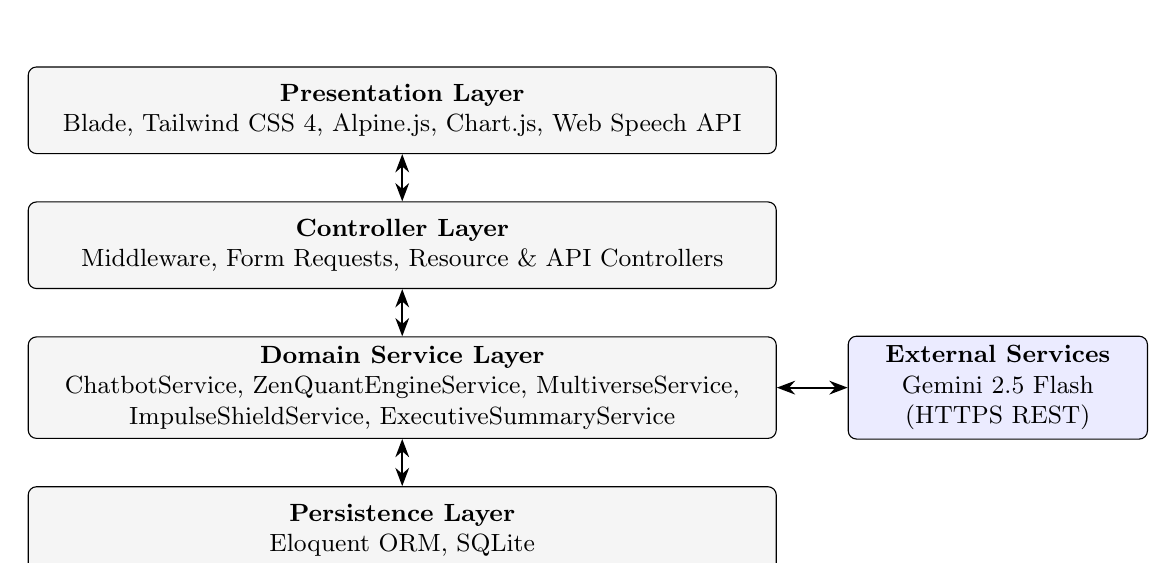
\begin{tikzpicture}[
  layer/.style={draw, rounded corners=3pt, minimum width=9.5cm, minimum height=1.1cm, align=center, font=\small, fill=gray!8},
  ext/.style={draw, rounded corners=3pt, minimum width=3.8cm, minimum height=1.1cm, align=center, font=\small, fill=blue!8},
  arr/.style={Stealth-Stealth, thick}]
\node[layer] (ui) {\textbf{Presentation Layer}\\ Blade, \TW{}, Alpine.js, Chart.js, Web Speech API};
\node[layer, below=0.6cm of ui] (ctl) {\textbf{Controller Layer}\\ Middleware, Form Requests, Resource \& API Controllers};
\node[layer, below=0.6cm of ctl] (svc) {\textbf{Domain Service Layer}\\ ChatbotService, ZenQuantEngineService, MultiverseService,\\ ImpulseShieldService, ExecutiveSummaryService};
\node[layer, below=0.6cm of svc] (orm) {\textbf{Persistence Layer}\\ Eloquent ORM, SQLite};
\node[ext, right=0.9cm of svc] (gem) {\textbf{External Services}\\ Gemini 2.5 Flash\\ (HTTPS REST)};
\draw[arr] (ui) -- (ctl);
\draw[arr] (ctl) -- (svc);
\draw[arr] (svc) -- (orm);
\draw[arr] (svc) -- (gem);
\end{tikzpicture}
\caption{Layered Architecture of FinSight AI}
\label{fig:arch}
\end{figure}

\begin{enumerate}[label=\arabic*.,leftmargin=*,itemsep=6pt]
\item \textbf{Presentation layer:}
Blade templates with \TW{} utilities and Alpine.js components, giving a dark/light glassmorphism interface. Chart.js canvases visualise cash flow, asset distribution, and 4-D budget consumption. A direct DOM ticker updates sub-paise cash flow at 60 FPS without reactive overhead.

\item \textbf{Controller layer:}
The HTTP kernel passes each request through authentication, email verification, sessions, and CSRF validation. Resource and API controllers (\texttt{ChatController}, \texttt{ZenQuantNexusController}, \texttt{MultiverseController}, \texttt{ImpulseShieldController}, \texttt{DashboardController}) handle business validation and return views or JSON payloads.

\item \textbf{Domain service layer:}
Reusable service classes encapsulate business rules, mathematical models, and external integrations:
\begin{itemize}[leftmargin=*]
    \item \texttt{ChatbotService}: intent extraction, conversational memory compilation, Gemini prompt dispatch, and 15-topic dynamic local fallback.
    \item \texttt{ZenQuantEngineService}: Financial Independence live telemetry ($V = C - B$), autonomous 3-agent Capital Council deliberation, 4-D radar analysis, and overnight sweep arbitrage.
    \item \texttt{MultiverseService}: branch creation, timeline cloning, financial delta diffing, and timeline merging.
    \item \texttt{ImpulseShieldService}: cooling-off vault timers, life-energy working hours conversion, and 10-year compounding regret calculations.
    \item \texttt{ExecutiveSummaryService} and \texttt{CompetitorAnalysisService}: automated briefings.
\end{itemize}

\item \textbf{Persistence layer:}
Eloquent ORM maps models to SQLite and enforces relationships (\texttt{hasMany}, \texttt{belongsTo}), type casting, Carbon date handling and mass-assignment protection.

\item \textbf{External generative AI gateway:}
HTTPS calls to Google's Generative Language API (\texttt{gemini-2.5-flash}) with structured JSON output configurations, system instructions, and dynamic user profiles.
\end{enumerate}


\subsection{Mathematical Formulations}\label{s422}

\textbf{1. Financial Independence Velocity and Live Telemetry ($V = C - B$).}
Let $A$ be total invested capital and $r = 12\%$ the expected annualized equity CAGR. The second-by-second passive capital compounding yield rate $C$ (with $T_{\text{sec}} = 365.25 \times 86400$) is
\begin{equation}
C = A \times \left[(1 + r)^{\frac{1}{T_{\text{sec}}}} - 1\right]
\end{equation}
Let $B_{\text{mo}}$ be monthly living expenditure. The per-second living burn rate $B$ is
\begin{equation}
B = \frac{B_{\text{mo}}}{30.4375 \times 86400}
\end{equation}
The net financial velocity $V$ is
\begin{equation}
V = C - B
\end{equation}
When $V > 0$, the user has achieved \textbf{Financial Independence Escape Velocity} (passive yield permanently exceeds living costs). When $V \le 0$, the system operates in the \textbf{Capital Accumulation Phase}. The target capital required for permanent financial independence under a safe withdrawal rate $r_{\text{safe}} = 4\%$ is
\begin{equation}
A_{\text{escape}} = \frac{12 \times B_{\text{mo}}}{r_{\text{safe}}} = 300 \times B_{\text{mo}}
\end{equation}
and the remaining capital gap is $\Delta A = \max\left(0, A_{\text{escape}} - A\right)$.

\textbf{2. 10-Year Compounding Opportunity Cost Formulation.}
For any discretionary purchase $P$ evaluated by the Capital Council or Impulse Shield, the 10-year compounding opportunity cost forfeiting Nifty 50 equity growth at $r = 12\%$ CAGR is
\begin{equation}
\text{Cost}_{\text{opp}} = P \times (1 + r)^{10} \approx P \times 3.1058
\end{equation}
Every rupee spent on transient lifestyle consumption sacrifices over three times its value in compounded decade-long wealth.

\textbf{3. Life-Energy Labor Hours (Impulse Shield Formulation).}
To confront impulsive spending with the real human cost of labor, purchase price $P$ is converted into working hours $H_{\text{labor}}$ based on monthly active income $I_{\text{tot}}$ assuming 160 working hours per month:
\begin{equation}
H_{\text{labor}} = \frac{P}{\text{Hourly Wage}} = \frac{P}{I_{\text{tot}} / 160} = \frac{160 \times P}{I_{\text{tot}}}
\end{equation}
For an income of Rs 50,000, a Rs 25,000 gadget demands 80 hours (two full work weeks) of labor.

\textbf{4. 4-D Capital Allocation Drag Ratio.}
Expenses are partitioned into four behavioral axes: Physical Essentials ($E_{\text{surv}}$), Growth \& Development ($E_{\text{soul}}$), Discretionary Leisure ($E_{\text{hedonic}}$), and Unplanned Miscellaneous ($E_{\text{chaos}}$). The Hedonic-to-Growth Drag Ratio $R_{\text{drag}}$ is
\begin{equation}
R_{\text{drag}} = \frac{E_{\text{hedonic}}}{\max(1, E_{\text{soul}})}
\end{equation}
Ratios $R_{\text{drag}} \le 0.5$ indicate \textbf{Disciplined Growth Equilibrium}, $0.5 < R_{\text{drag}} \le 1.5$ represent \textbf{Moderate Equilibrium}, and $R_{\text{drag}} > 1.5$ trigger \textbf{High Hedonic Drag Alerts}.

\textbf{5. FinScore (0--1000 financial health indicator).}
Let $I_{\text{tot}}$ be total income, $E_{\text{tot}}$ total expenses and $N_{\text{goals}}$ the number of active goals. For $I_{\text{tot}} > 0$ the savings rate $S_r$ and expense ratio $E_r$ are
\begin{equation}
S_r = \frac{I_{\text{tot}} - E_{\text{tot}}}{I_{\text{tot}}} \times 100, \qquad E_r = \frac{E_{\text{tot}}}{I_{\text{tot}}} \times 100
\end{equation}
and the score $\Phi$ is
\begin{equation}
\Phi = \max\left(0, \min\left(1000, \, \operatorname{round}\left(700 + 2.5\,S_r + 10\,N_{\text{goals}} - P(E_r)\right)\right)\right)
\end{equation}
\begin{equation}
P(E_r) = \begin{cases} 50, & E_r > 80 \\ 0, & \text{otherwise} \end{cases}
\end{equation}

\textbf{6. Least-squares linear regression for cash flow forecasting.}
For the last $n = 6$ months, let $x_i \in \{1,\dots,6\}$ be the month index and $y_i$ the monthly net cash flow. The model is $\hat{y} = mx + c$ with
\begin{equation}
m = \frac{n \sum x_i y_i - \left(\sum x_i\right)\left(\sum y_i\right)}{n \sum x_i^2 - \left(\sum x_i\right)^2}, \qquad
c = \frac{\sum y_i - m \sum x_i}{n}
\end{equation}
and the forecast for the next three months $k \in \{1,2,3\}$ is $\hat{y}_{n+k} = \max\left(0, \, c + m(n + k)\right)$.\cite{linear_regression}


\subsection{Worked Example: Regression Forecast}\label{s4221}

The following illustrative data show the calculation. Take six months of net cash flow, in Rs: 42,000; 45,000; 43,000; 48,000; 50,000; 52,000.

With $\sum x = 21$, $\sum x^2 = 91$, $\sum y = 2{,}80{,}000$ and $\sum xy = 10{,}15{,}000$:
\begin{align*}
m &= \frac{6(10{,}15{,}000) - 21(2{,}80{,}000)}{6(91) - 21^2} = \frac{2{,}10{,}000}{105} = 2{,}000\\
c &= \frac{2{,}80{,}000 - 2{,}000(21)}{6} \approx 39{,}666.67
\end{align*}
The forecast for months 7, 8 and 9 is therefore Rs 53,666.67, Rs 55,666.67 and Rs 57,666.67.

\textbf{Accuracy check.} On the six fitted points the mean absolute error is about Rs 889 (about 2\% of the values) and $R^2 \approx 0.88$. Fitting the first five months yields $m = 1{,}900$ and $c = 39{,}900$, projecting Rs 51,300 for month 6 against an actual Rs 52,000 (1.3\% error).

\textbf{Time Machine.} If the user introduces a Rs 15,000 monthly commitment, the simulator subtracts it from each projected month, so month 7 drops from Rs 53,666.67 to Rs 38,666.67.


\subsection{Database Design}\label{s4222}

The relational schema has one parent table (\texttt{users}) and nine child tables, each holding a \texttt{user\_id} foreign key with cascading delete. Figure~\ref{fig:er} illustrates the entity relationships and Table~\ref{tab:schema} lists the key attributes, satisfying third normal form (3NF).

\begin{figure}[H]
\centering
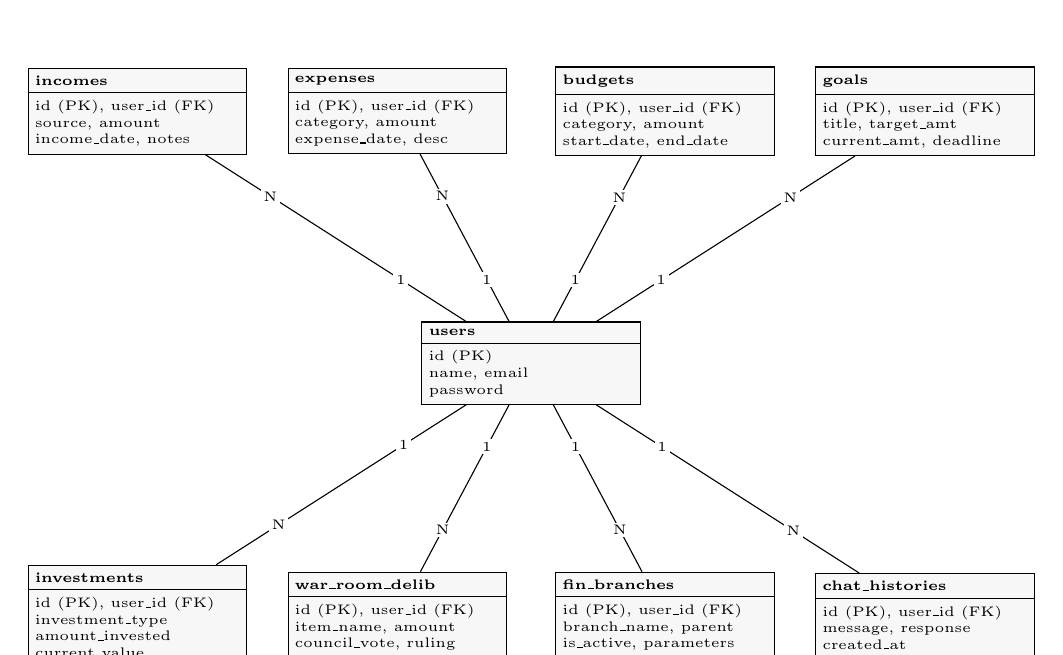
\begin{tikzpicture}[
  ent/.style={draw, rectangle split, rectangle split parts=2, font=\tiny, text width=2.6cm, align=left, fill=gray!6, inner sep=2.5pt},
  card/.style={font=\tiny, fill=white, inner sep=1pt}]
\node[ent] (users) at (0,0) {\textbf{users}\nodepart{second}id (PK)\\name, email\\password};
\node[ent] (inc) at (-5.0,3.2) {\textbf{incomes}\nodepart{second}id (PK), user\_id (FK)\\source, amount\\income\_date, notes};
\node[ent] (exp) at (-1.7,3.2) {\textbf{expenses}\nodepart{second}id (PK), user\_id (FK)\\category, amount\\expense\_date, desc};
\node[ent] (bud) at (1.7,3.2) {\textbf{budgets}\nodepart{second}id (PK), user\_id (FK)\\category, amount\\start\_date, end\_date};
\node[ent] (goa) at (5.0,3.2) {\textbf{goals}\nodepart{second}id (PK), user\_id (FK)\\title, target\_amt\\current\_amt, deadline};
\node[ent] (inv) at (-5.0,-3.2) {\textbf{investments}\nodepart{second}id (PK), user\_id (FK)\\investment\_type\\amount\_invested\\current\_value};
\node[ent] (war) at (-1.7,-3.2) {\textbf{war\_room\_delib}\nodepart{second}id (PK), user\_id (FK)\\item\_name, amount\\council\_vote, ruling};
\node[ent] (bra) at (1.7,-3.2) {\textbf{fin\_branches}\nodepart{second}id (PK), user\_id (FK)\\branch\_name, parent\\is\_active, parameters};
\node[ent] (cha) at (5.0,-3.2) {\textbf{chat\_histories}\nodepart{second}id (PK), user\_id (FK)\\message, response\\created\_at};
\foreach \c in {inc,exp,bud,goa,inv,war,bra,cha}
  \draw (users) -- node[card, near start]{1} node[card, near end]{N} (\c);
\end{tikzpicture}
\caption{Entity--Relationship Diagram of FinSight AI}
\label{fig:er}
\end{figure}

\begin{table}[H]
\centering
\caption{Representative Database Schema}
\label{tab:schema}
\footnotesize
\renewcommand{\arraystretch}{1.2}
\begin{tabular}{|p{3.2cm}|p{7.2cm}|p{3.2cm}|}
\hline
\textbf{Table} & \textbf{Main attributes} & \textbf{Relationship} \\ \hline
\texttt{users} & id, name, email, password, timestamps & parent of all entities \\ \hline
\texttt{incomes} & user\_id, source, amount (decimal), income\_date, notes & belongs to user \\ \hline
\texttt{expenses} & user\_id, category, amount (decimal), expense\_date, description & belongs to user \\ \hline
\texttt{budgets} & user\_id, category, amount, start\_date, end\_date & belongs to user \\ \hline
\texttt{goals} & user\_id, title, target\_amount, current\_amount, deadline & belongs to user \\ \hline
\texttt{investments} & user\_id, investment\_type, amount\_invested, current\_value & belongs to user \\ \hline
\texttt{war\_room\_deliberations} & user\_id, item\_name, amount, category, user\_justification, kenji\_argument, chen\_argument, minjun\_argument, council\_vote, final\_ruling & belongs to user \\ \hline
\texttt{financial\_branches} & user\_id, branch\_name, parent\_branch, is\_active, scenario\_parameters & belongs to user \\ \hline
\texttt{impulse\_vault\_items} & user\_id, item\_name, amount, unlock\_at, status & belongs to user \\ \hline
\texttt{chat\_histories} & user\_id, message, response, timestamps & belongs to user \\ \hline
\end{tabular}
\end{table}


\subsection{Use Case Diagram}\label{s423}

The use case diagram illustrates how authenticated users and the external Gemini service interact with the system across telemetry, multi-agent council deliberations, multiverse timelines, and transaction logging.

\begin{figure}[H]
\centering
\IfFileExists{usecase.png}{
\includegraphics[width=0.90\textwidth]{usecase.png}
}{
\fbox{\parbox[c][6.5cm][c]{0.85\textwidth}{
\centering \textbf{[ FinSight AI Use Case Diagram Placeholder ]}\\
\vspace{0.4cm}
\small Actors: Authenticated User, External Gemini LLM.\\
Use cases: Transaction Logging, War Room Council, Telemetry Simulation, Multiverse Branching, Impulse Shield, FinScore, 80C Tax Audit.\\
\vspace{0.2cm}
\textit{Upload usecase.png to Overleaf}
}}
}
\caption{Use Case Diagram of FinSight AI}
\label{fig:usecase}
\end{figure}


\subsection{Activity Diagram}\label{s424}

The activity diagram traces the execution lifecycle from user authentication to live telemetry calculation, natural language transaction parsing, and AI deliberation.

\begin{figure}[H]
\centering
\IfFileExists{activity.png}{
\includegraphics[width=0.80\textwidth]{activity.png}
}{
\fbox{\parbox[c][6.5cm][c]{0.85\textwidth}{
\centering \textbf{[ FinSight AI Activity Diagram Placeholder ]}\\
\vspace{0.4cm}
\small Login $\rightarrow$ Telemetry Computation ($V=C-B$) $\rightarrow$ Intent Detection $\rightarrow$ Database Update $\rightarrow$ Council Audit $\rightarrow$ Cached Briefing.\\
\vspace{0.2cm}
\textit{Upload activity.png to Overleaf}
}}
}
\caption{Activity Diagram of FinSight AI}
\label{fig:activity}
\end{figure}


\section{Modules or Functional Description}\label{s43}

\subsection{User Authentication and Security}\label{s431}
Built on Laravel Breeze, this module provides bcrypt password hashing, session management, email verification, password reset and login throttling. All routes sit behind the \texttt{auth} middleware, and queries are strictly scoped to the signed-in user.

\subsection{Income Stream Management}\label{s432}
Users record salary, freelance, consulting, dividend and rental income with source, amount, date and notes. Eloquent aggregates give total and period-specific income for cash flow calculations.

\subsection{Expense Categorization}\label{s433}
Expenses are logged by date, category, amount and note across categories such as Housing, Utilities, Groceries, Dining, Transportation, Healthcare and Entertainment, feeding budget and telemetry monitors.

\subsection{Smart Budget Planner}\label{s434}
Users set monthly caps per category. Utilisation is tracked dynamically, displaying colour-coded warnings from cyan to amber to red as spending nears or exceeds the limit.

\subsection{Goal Milestone Tracking}\label{s435}
For goals such as an emergency fund or a down payment, users set a target, starting amount and deadline, tracking progress percentages and passing active goals to the FinScore and AI advisor.

\subsection{Investment Portfolio Management}\label{s436}
Tracks principal invested and current value across equities, mutual funds, gold, real estate and government schemes (PPF, EPF, NPS), calculating capital gains and linking to Section 80C.

\subsection{The Zen \& Quant Nexus: Financial Independence Telemetry}\label{s437}
This module implements a real-time financial physics engine calculating net capital accumulation velocity ($V = C - B$) in Indian Rupees per second. A 60 FPS sub-paise odometer visualises continuous capital compounding versus living burn rate with direct DOM mutation. An interactive parameter tuning drawer allows users to simulate changes to monthly expenses, portfolio size, and expected CAGR in real time.

\subsection{The Autonomous AI Capital Council (War Room Deliberation)}\label{s438}
Before high-ticket or discretionary card swipes, users summon an autonomous AI council that evaluates proposals across three objective dimensions:
\begin{enumerate}[leftmargin=*]
    \item \textbf{Behavioral \& Mindful Audit:} Evaluates intentionality, psychological clutter, and hedonic treadmill adaptation risks.
    \item \textbf{Quantitative Opportunity Cost:} Analyzes 10-year compounding wealth impact ($P \times (1+r)^{10}$ in Nifty 50 at 12\% CAGR) and capital velocity drag.
    \item \textbf{Productivity \& Growth ROI:} Measures time leverage, career velocity, and practical utility multiplier.
\end{enumerate}
The council issues actionable verdicts: \textbf{APPROVED}, \textbf{VETOED}, or \textbf{CONDITIONAL} (e.g., matching 50\% into liquid index funds), persisting deliberations for review.

\subsection{The 4-D Capital Allocation Radar}\label{s439}
Classifies all expenses into four behavioral axes: Physical Essentials, Growth \& Development, Discretionary Leisure, and Unplanned Miscellaneous. Rendered via Chart.js Radar, it computes the Hedonic-to-Growth Drag Ratio, flagging lifestyle creep with disciplined equilibrium badges.

\subsection{Automated Overnight Cash Sweep}\label{s4310}
Detects idle cash sitting in low-yield savings accounts (2.7\%) above a 30-day operating buffer (Rs 35,000) and calculates the cost of inaction. A stateful 1-click virtual sweep simulates sweeping surplus liquidity into AAA overnight liquid yields (+4.5\% spread), dynamically feeding the live telemetry engine.

\subsection{The Financial Multiverse (``Git for Your Money'')}\label{s4311}
Enables users to branch parallel financial timelines from their main ledger (e.g., sabbatical, startup launch, property purchase). Users can perform financial diffing (net worth delta, savings rate delta, cash flow divergence), chat with an alternate timeline advisor, and merge hypothetical scenarios into their primary plan.

\subsection{The Impulse Shield \& 48-Hour Temptation Vault}\label{s4312}
A behavioral pre-commitment tool for cooling off impulse purchases. The system converts the item's price into life-energy working hours ($H_{\text{labor}}$) and calculates 10-year compounding regret. Items enter a strict 48-hour vault countdown before execution is permitted.

\subsection{Frictionless Data Ingestion: UPI SMS Auto-Parser}\label{s4313}
To eliminate manual data-entry friction, users paste raw bank or UPI transactional SMS messages (HDFC, SBI, ICICI, Axis, Paytm, PhonePe, GPay). A regex NLP pipeline automatically extracts the amount, merchant, transaction type, and date, populating categorized expense records instantly.

\subsection{JARVIS Voice CFO}\label{s4314}
A voice-driven financial assistant using the Web Speech API. Users tap an interactive floating orb to speak financial queries or log transactions, watching an animated canvas soundwave visualizer and hearing spoken financial summaries.

\subsection{Resilient Multi-Topic AI Financial Advisor}\label{s4315}
The conversational advisor compiles a live profile and the last four conversational turns to deliver cohesive, context-aware financial advice. To prevent repetitive answers, prompt directives enforce topic-first responses without reciting redundant goal congratulations. When offline, a 15-topic dynamic fallback engine computes real numbers for gold, stocks, mutual funds, expenses, debt, emergency funds, and taxes.

\subsection{Dual-Persona Engine}\label{s4316}
A chat toggle switches between two AI personas: \textbf{Professional mode} (structured, encouraging, tactical) and \textbf{Roast mode} (sarcastic, humorous critique of lifestyle leaks that delivers harsh financial truths).

\subsection{Predictive Cash Flow Forecasting}\label{s4317}
Using least-squares regression over six months of history, the module projects income, expenses and net balance for the next three months and plots them on a Chart.js canvas.

\subsection{Scenario Simulator (``Time Machine'')}\label{s4318}
Allows users to add hypothetical monthly commitments (e.g., Rs 15,000 EMI) and dynamically redraws the projected cash flow balance.

\subsection{Hidden Subscription Hunter}\label{s4319}
Scans rolling 90-day expenses for identical amounts recurring in the same category at least 20 days apart, displaying annual leakages on the dashboard.

\subsection{Tax Optimization (Section 80C) Analyzer}\label{s4320}
Totals qualifying tax-saving investments (ELSS, PPF, EPF) against the Rs 1,50,000 threshold and highlights the remaining tax-saving gap under the old regime.

\subsection{Competitor Intelligence and Rental Benchmarking}\label{s4321}
Allows property owners to benchmark rent and occupancy against local competitors, generating an AI market briefing via \texttt{CompetitorAnalysisService}.

\subsection{Reporting and Executive Summary}\label{s4322}
Generates formal financial statements with cached AI briefings (1-hour TTL) summarizing savings rates, spending drivers, and risk factors.

\subsection{Responsive Glassmorphism Interface}\label{s4323}
Uses \TW{} and CSS variables for a modern glassmorphism aesthetic with theme persistence and zero FOUC on page load.


\section{Implementation Performed}\label{s44}

The application was built systematically layer by layer.

\textbf{Backend and Database Architecture.} Built on \LV{}, PHP 8.3, and SQLite with foreign-key cascades, decimal precision for currency, and indexes on \texttt{user\_id} and date columns.

\textbf{High-Performance Telemetry Engine.} To render a 60 FPS millisecond counter without browser lag, the accumulator ticker directly updates DOM \texttt{textContent} on an interval timer, completely bypassing Alpine.js reactive proxies to ensure 0\% CPU thrashing.

\textbf{Generative AI \& Multi-Agent Deliberation.} \texttt{ZenQuantEngineService} calls Gemini 2.5 Flash with structured JSON schemas to extract multi-perspective council arguments and votes. \texttt{ChatbotService} maintains conversational context by injecting the last four conversation exchanges and enforcing topic-first guidelines with temperature 0.75.

\textbf{Prioritized Intent Parsing.} Regular expressions in \texttt{detectAndExecuteAction()} evaluate budgets first, incomes second, and expenses third, with keyword guards preventing misclassification.


\section{Testing and Validation}\label{s441}

The application was validated through an automated PHPUnit test suite consisting of \textbf{57 automated tests and 215 assertions} with a 100\% pass rate, combined with systematic browser validation. Table~\ref{tab:tests} summarizes key test cases.

\begingroup
\singlespacing
\footnotesize
\setlength{\tabcolsep}{4pt}
\renewcommand{\arraystretch}{1.15}
\setlength{\parskip}{0pt}
\begin{longtable}{|p{0.9cm}|p{2.4cm}|p{4.2cm}|p{4.3cm}|p{1.5cm}|}
\caption{Test Cases}\label{tab:tests}\\
\hline \textbf{ID} & \textbf{Module} & \textbf{Input / Action} & \textbf{Expected result} & \textbf{Status} \\ \hline
\endfirsthead
\hline \textbf{ID} & \textbf{Module} & \textbf{Input / Action} & \textbf{Expected result} & \textbf{Status} \\ \hline
\endhead
TC1 & Authentication & Open \texttt{/dashboard} without logging in & Redirect to login page & Pass \\ \hline
TC2 & Authorization & User A requests an expense belonging to User B & Denied (403/404) & Pass \\ \hline
TC3 & CSRF & POST expense form without token & Rejected with HTTP 419 & Pass \\ \hline
TC4 & Expense Valid & Submit negative or empty amount & Validation error, rejected & Pass \\ \hline
TC5 & Chat Intent & ``5000 as petrol expense'' & Recorded Rs 5,000 under Petrol & Pass \\ \hline
TC6 & Chat Intent & ``add Rs 45000 salary income'' & Recorded Rs 45,000 from Salary & Pass \\ \hline
TC7 & Chat Intent & ``set budget of Rs 5000 for food'' & Budget of Rs 5,000 for Food & Pass \\ \hline
TC8 & AI Fallback & Ask about gold with API offline & SGB and Gold ETF advice & Pass \\ \hline
TC9 & AI Fallback & Ask about savings with API offline & 50/30/20 advice with real savings rate & Pass \\ \hline
TC10 & Forecast & Six months: 42k, 45k, 43k, 48k, 50k, 52k & $m = 2000$; month 7 $\approx$ 53,666.67 & Pass \\ \hline
TC11 & Forecast & No historical data & Forecast of zeros, no exception & Pass \\ \hline
TC12 & FinScore & Income 1,00,000, expenses 70,000, 3 goals & Score 805 & Pass \\ \hline
TC13 & FinScore & User with no income recorded & ``N/A'' shown & Pass \\ \hline
TC14 & Subscriptions & Rs 649 charged twice, 30 days apart & Flagged, annual cost 7,788 & Pass \\ \hline
TC15 & Section 80C & ELSS 50,000 and PPF 40,000 & Shortfall of 60,000 & Pass \\ \hline
TC16 & Telemetry API & GET \texttt{/api/nexus/telemetry} & Returns velocity, burn, gap & Pass \\ \hline
TC17 & War Room & POST proposal for headphones (Rs 24,990) & Returns 3 arguments and vote & Pass \\ \hline
TC18 & Multiverse & Create timeline branch ``Sabbatical'' & Clones state and isolates diffs & Pass \\ \hline
TC19 & Impulse Vault & Lock Rs 15,000 watch for 48 hours & Converts to labor hours and locks & Pass \\ \hline
TC20 & SMS Parser & Paste standard UPI debit alert SMS & Auto-extracts amount and merchant & Pass \\ \hline
TC21 & Chat Investment & ``add investment 50000 in ELSS'' & Recorded Rs 50,000 ELSS holding & Pass \\ \hline
TC22 & Investment KPI & Authenticated user visits \texttt{/investments} & Evaluates telemetry cards \& ROI & Pass \\ \hline
\end{longtable}
\endgroup


\section{Screenshots of Work}\label{s45}

The figures below illustrate the core interfaces of FinSight AI.

\begin{figure}[H]
\centering
\shot{dashboard.png}{0.95}{5cm}{FinSight AI Real-Time Dashboard}{FinScore gauge, KPI cards, forecast chart and subscription alert.}
\caption{FinSight AI Real-Time Dashboard}
\end{figure}

\begin{figure}[H]
\centering
\shot{nexus_dashboard.png}{0.95}{5cm}{The Zen \& Quant Nexus}{Financial independence telemetry, 60 FPS sub-paise accumulator, parameter tuning simulator, 4-D capital radar, and overnight cash sweep.}
\caption{The Zen \& Quant Nexus Telemetry \& Arbitrage Suite}
\end{figure}

\begin{figure}[H]
\centering
\shot{war_room_council.png}{0.95}{5cm}{Autonomous Capital Council Deliberation}{Multi-perspective pre-purchase audit: Behavioral, Quantitative Opportunity Cost, and Productivity ROI.}
\caption{Autonomous AI Capital Council Deliberation Chamber}
\end{figure}

\begin{figure}[H]
\centering
\shot{multiverse_branches.png}{0.95}{5cm}{The Financial Multiverse}{Timeline branching, scenario diffing, and alternate timeline advisor chat.}
\caption{The Financial Multiverse Timeline Branching}
\end{figure}

\begin{figure}[H]
\centering
\shot{impulse_shield.png}{0.95}{5cm}{The Impulse Shield}{48-hour temptation vault, life-energy working hours converter, and 10-year compounding regret.}
\caption{The Impulse Shield \& Temptation Vault}
\end{figure}

\begin{figure}[H]
\centering
\shot{cashflow_forecast.png}{0.95}{5cm}{Cash Flow Forecast and Scenario Simulator}{Six months of actuals, three-month regression forecast and the Time Machine EMI simulator.}
\caption{Cash Flow Forecast and Scenario Simulator}
\end{figure}

\begin{figure}[H]
\centering
\shot{chat_advisor.png}{0.95}{5cm}{AI Financial Advisor}{Gemini chat interface with conversational memory, dynamic guidance, and action badges.}
\caption{FinSight AI Conversational Advisor}
\end{figure}

\begin{figure}[H]
\centering
\shot{nlp_action.png}{0.95}{5cm}{Natural Language Transaction Logging}{Command such as ``5000 as petrol expense'' and automated record creation.}
\caption{Intent Detection and Automated Transaction Logging}
\end{figure}

\begin{figure}[H]
\centering
\shot{roast_mode.png}{0.95}{5cm}{Roast Mode}{Roast Mode toggle with sarcastic feedback on spending habits.}
\caption{FinSight AI Chatbot in Roast Mode}
\end{figure}

\begin{figure}[H]
\centering
\shot{voice_cfo.png}{0.95}{5cm}{JARVIS Voice CFO}{Web Speech API voice interaction with interactive soundwave visualizer.}
\caption{JARVIS Voice CFO Interactive Interface}
\end{figure}

\begin{figure}[H]
\centering
\shot{budgets.png}{0.95}{5cm}{Budget Planner}{Category limits with colour-coded progress bars.}
\caption{Category Budget Planner}
\end{figure}

\begin{figure}[H]
\centering
\shot{goals.png}{0.95}{5cm}{Goal Tracking}{Progress, target and current amounts for each goal.}
\caption{Financial Goal Tracking}
\end{figure}

\begin{figure}[H]
\centering
\shot{investments.png}{0.95}{5cm}{Investment Portfolio}{Allocations, invested capital, current value and Section 80C tags.}
\caption{Investment Portfolio Management}
\end{figure}

\begin{figure}[H]
\centering
\shot{reports.png}{0.95}{5cm}{Reports and AI Summary}{Financial statement, category breakdown and cached AI summary.}
\caption{Financial Reports and AI Executive Summary}
\end{figure}

\begin{figure}[H]
\centering
\shot{competitors.png}{0.95}{5cm}{Competitor Benchmarking}{Rent and occupancy benchmarks with the Gemini briefing.}
\caption{Competitor Intelligence and Market Benchmarking}
\end{figure}

% ===================== CHAPTER 5 =====================
\chapter{Learning Outcomes}\label{ch5}

\section{Skills Acquired}\label{s51}

The internship at CodeDesign Technologies was a valuable milestone in my technical development. Building FinSight AI gave me the following competencies:

\subsection{Backend Framework and Architecture}
Proficiency in PHP 8.3 and \LV{}, mastering MVC design, dependency injection, service layers, Eloquent ORM, database migrations, mass-assignment protection, and automated PHPUnit testing.

\subsection{Generative AI and Multi-Agent Prompt Engineering}
Designing structured prompts with JSON schema outputs, multi-turn conversation memory pipelines, temperature optimization, rate-limit resilience, and graceful multi-topic local fallbacks.

\subsection{Real-Time Financial Physics and High-Performance DOM}
Mathematical modeling of continuous compounding yield versus living burn velocity ($V = C - B$), and implementing 60 FPS sub-paise odometers using direct DOM mutation to eliminate reactive CPU throttling.

\subsection{Natural Language Processing and Intent Extraction}
Building regular expression pipelines with priority ordering to extract monetary figures, categories, and relative dates from free-form chat and Indian bank SMS alerts.

\subsection{Mathematical and Predictive Modelling}
Implementing ordinary least-squares regression, 10-year compounding opportunity cost formulas, life-energy labor hours conversion, and heuristic scoring models.

\subsection{Frontend Engineering}
Advanced styling with \TW{}, reactive client states with Alpine.js, interactive visualisations with Chart.js, and speech interaction with the Web Speech API.


\section{Knowledge Gained}\label{s52}

\begin{itemize}[leftmargin=*]
    \item \textbf{Financial domain depth:} cash flow velocity, financial escape velocity, compounding opportunity costs, 4-D budget allocation, and tax optimization.
    \item \textbf{Separation of concerns:} decoupling business calculations into dedicated service classes for high testability.
    \item \textbf{High-frequency UI performance:} understanding browser repaint cycles and why direct DOM manipulation outperforms reactive virtual DOM bindings for sub-second updates.
    \item \textbf{Graceful degradation:} engineering multi-layered local fallback engines ensuring uninterrupted operation during cloud API downtime.
\end{itemize}


\section{Challenges Faced and Solutions}\label{s53}

\begin{table}[H]
\centering
\caption{Challenges Faced and Solutions Implemented}
\renewcommand{\arraystretch}{1.3}
\begin{tabular}{|p{6.0cm}|p{8.0cm}|}
\hline
\textbf{Challenge} & \textbf{Solution} \\ \hline
60 FPS millisecond counter causing severe browser CPU thrashing with reactive frameworks
&
Direct DOM textContent mutations (\texttt{odometerDisplay.textContent}) decoupled from Alpine.js proxies, achieving 0\% CPU lag.
\\ \hline
Repetitive AI conversational outputs and obsessive goal congratulations
&
Injecting the last four conversation exchanges into prompt context, adding strict anti-repetition instructions, and building a 15-topic dynamic local fallback engine.
\\ \hline
Cross-matching collisions in natural language intent parsing
&
Reordered regex detection to evaluate budgets first, incomes second, and expenses third, with keyword exclusion guards.
\\ \hline
High friction in manual transaction logging
&
Implemented UPI SMS auto-parser extracting amount, merchant, and category from raw bank SMS notifications.
\\ \hline
Cloud AI latency and network timeouts
&
A 25-second HTTP timeout with \texttt{try-catch} error handling and a 15-topic dynamic rule-based fallback.
\\ \hline
Theme flash on initial page load
&
An inline \texttt{<x-theme-init>} component in the document head reading \texttt{localStorage} before DOM paint.
\\ \hline
\end{tabular}
\end{table}


\section{Relevance of the Work}\label{s54}

The project links directly to core MCA subjects:
\begin{enumerate}[leftmargin=*]
    \item \textbf{Advanced Web Technologies:} server-side frameworks, client-side reactivity, REST conventions, asset bundling, and Web Speech API.
    \item \textbf{Database Management Systems:} relational schema design, 3NF normalisation, foreign-key cascades, and aggregated queries.
    \item \textbf{Software Engineering:} SDLC, MVC, defensive coding, and 57 automated PHPUnit test suites.
    \item \textbf{Artificial Intelligence and Machine Learning:} prompt engineering, multi-agent structured JSON decoding, and linear regression modelling.
\end{enumerate}


% ===================== CHAPTER 6 =====================
\chapter{Limitations, Future Scope and Conclusion}\label{ch6}

\section{Limitations}\label{s60}

\begin{itemize}[leftmargin=*]
    \item The financial independence velocity engine assumes a constant 12\% equity CAGR and steady living burn, not accounting for short-term market drawdowns.
    \item Linear regression forecasting fits a straight-line trend to six data points without modeling seasonality or providing statistical confidence intervals.
    \item The FinScore heuristic uses expert judgement weights rather than empirical fitting.
    \item Natural language intent parsing relies on regular expressions; atypical sentence phrasing falls through to the general AI chat.
    \item Section 80C tracking reflects the old tax regime and requires section renumbering under the Income-tax Act, 2025.
    \item Transactions are entered manually, via chat, or through SMS paste; there is currently no direct Account Aggregator banking API integration.
\end{itemize}


\section{Future Enhancements}\label{s61}

\begin{itemize}[leftmargin=*]
    \item \textbf{Account Aggregator Integration:} Connecting with RBI-regulated Account Aggregators for automated, consent-based bank statement sync.
    \item \textbf{Receipt OCR:} Machine-vision extraction of items and totals from photographed physical receipts.
    \item \textbf{Monte Carlo Financial Physics:} Upgrading the velocity engine with 10,000-path stochastic Monte Carlo simulations to model sequence-of-returns risk.
    \item \textbf{Mobile Apps:} Native Flutter or React Native mobile applications with background push notifications for budget alerts and impulse vault releases.
    \item \textbf{Production Deployment:} Containerized Docker deployment with PostgreSQL, Redis cache, and CI/CD pipelines on AWS or GCP.
\end{itemize}


\section{Conclusion}\label{s62}

My 45-day internship at CodeDesign Technologies under the Summer Industry Immersion Programme was a transformative experience, connecting academic computer science principles with professional software engineering practice.

These skills culminated in \textbf{FinSight AI}, an advanced personal finance and predictive analytics platform built with \LV{}, PHP 8.3, SQLite, \TW{}, Alpine.js, and Chart.js. Beyond conventional passive ledgers, FinSight AI incorporates real-time financial independence telemetry ($V = C - B$), an autonomous multi-perspective AI Capital Council, a Financial Multiverse for parallel timeline branching, a 48-hour behavioral Impulse Shield, UPI SMS parsing, and Gemini-powered conversational intelligence with resilient 15-topic dynamic fallbacks.

The programme significantly enhanced my technical proficiency, algorithmic problem-solving, and software craftsmanship, providing a solid foundation for my future career in full-stack engineering and applied artificial intelligence.


% ===================== CHAPTER 7 =====================
\clearpage
\chapter{Bibliography}\label{refs}
\section{References}\label{s71}
\vspace{-0.5cm}
\begingroup
\raggedright
\sloppy
\setlength{\parskip}{0pt}

\begin{thebibliography}{99}

\bibitem{codedesign}
CodeDesign Technologies Pvt Ltd. \textit{About Us}. \url{https://codedesign.in/about-us.php}

\bibitem{laravel}
Laravel. \textit{Laravel Documentation}. \url{https://laravel.com/docs}

\bibitem{php83}
The PHP Group. \textit{PHP Manual}. \url{https://www.php.net/manual/en/}

\bibitem{gemini}
Google. \textit{Gemini API Documentation}. \url{https://ai.google.dev/gemini-api/docs}

\bibitem{sqlite}
SQLite. \textit{SQLite Documentation}. \url{https://www.sqlite.org/docs.html}

\bibitem{tailwind}
Tailwind Labs. \textit{Tailwind CSS Documentation}. \url{https://tailwindcss.com/docs}

\bibitem{alpine}
Alpine.js. \textit{Alpine.js Documentation}. \url{https://alpinejs.dev}

\bibitem{chartjs}
Chart.js contributors. \textit{Chart.js Documentation}. \url{https://www.chartjs.org/docs/latest/}

\bibitem{vite}
Vite contributors. \textit{Vite Guide}. \url{https://vite.dev/guide/}

\bibitem{cleancode}
Robert C. Martin. \textit{Clean Architecture: A Craftsman's Guide to Software Structure and Design}. Prentice Hall, 2017.

\bibitem{incometax}
Income Tax Department, Government of India. \textit{Income Tax Portal}. \url{https://incometaxindia.gov.in}

\bibitem{linear_regression}
Douglas C. Montgomery, Elizabeth A. Peck, and G. Geoffrey Vining. \textit{Introduction to Linear Regression Analysis}, 5th ed. John Wiley \& Sons, 2012.

\end{thebibliography}
\endgroup


% ===================== CHAPTER 8 =====================
\clearpage
\chapter{Appendix}\label{appx}

\section{Sample Source Code}\label{s81}

This section lists representative extracts: natural language intent parsing with dynamic fallback, the Financial Independence Telemetry and War Room Council engine, and regression forecasting.

\subsection*{1. Intent Parser \& Dynamic Fallback (ChatbotService.php)}

\begin{lstlisting}[language=PHP]
protected function detectAndExecuteAction(User $user, string $message): ?array
{
    $lower = strtolower($message);

    // 1. Budget detection
    if (preg_match('/(?:create|set|add)\s+(?:a\s+)?(?:rs\.?\s*|₹\s*)?(\d[\d,]*(?:\.\d{1,2})?)\s*(?:rs\.?|rupees?)?\s+budget\s+(?:for\s+|on\s+)?([a-z ]+)/i', $message, $m)) {
        $amount = (float) str_replace(',', '', $m[1]);
        $category = ucfirst(trim($m[2]));
        $budget = $user->budgets()->create([
            'category' => $category, 'amount' => $amount,
            'start_date' => now()->startOfMonth(), 'end_date' => now()->endOfMonth(),
        ]);
        return ['type' => 'budget_created', 'label' => "Budget of Rs $amount for $category created."];
    }

    // 2. Income detection
    if (preg_match('/(?:add|received?|got|earned?|record)\s+(?:rs\.?\s*|₹\s*)?(\d[\d,]*(?:\.\d{1,2})?)\s*(?:rs\.?|rupees?)?\s+(?:as\s+|from\s+|via\s+)?([a-z ]+?)\s+income/i', $message, $m)) {
        $amount = (float) str_replace(',', '', $m[1]);
        $source = ucfirst(trim($m[2]));
        $income = $user->incomes()->create(['source' => $source, 'amount' => $amount, 'income_date' => now()]);
        return ['type' => 'income_created', 'label' => "Income of Rs $amount from $source recorded."];
    }

    // 3. Expense detection (guarded against income/budget keywords)
    if (!str_contains($lower, 'income') && !str_contains($lower, 'budget') &&
        preg_match('/(?:rs\.?\s*|₹\s*)?(\d[\d,]*(?:\.\d{1,2})?)\s*(?:rs\.?|rupees?)?\s+(?:as|for|on)\s+([a-z ]+?)(?:\s+expense)?$/i', $message, $m)) {
        $amount = (float) str_replace(',', '', $m[1]);
        $category = ucfirst(trim($m[2]));
        $expense = $user->expenses()->create(['category' => $category, 'amount' => $amount, 'expense_date' => now()]);
        return ['type' => 'expense_created', 'label' => "Expense of Rs $amount under $category recorded."];
    }
    return null;
}
\end{lstlisting}

\subsection*{2. Financial Independence Telemetry \& War Room (ZenQuantEngineService.php)}

\begin{lstlisting}[language=PHP]
public function calculateLiveTelemetry(User $user, ?float $customBurn = null, ?float $customAssets = null, float $cagr = 0.12): array
{
    $monthlyBurn = $customBurn ?? (float) $user->expenses()->sum('amount');
    if ($monthlyBurn <= 0) $monthlyBurn = 35000;

    $investedAssets = $customAssets ?? (float) $user->investments()->sum('current_value');

    // Yield per second at expected CAGR: C = A * ((1 + r)^(1/T) - 1)
    $secondsPerYear = 365.25 * 86400;
    $yieldPerSec = $investedAssets * (pow(1 + $cagr, 1 / $secondsPerYear) - 1);

    // Burn per second: B = monthlyBurn / secondsInMonth
    $burnPerSec = $monthlyBurn / (30.4375 * 86400);

    // Net Velocity: V = C - B
    $netVelocity = $yieldPerSec - $burnPerSec;
    $capitalForEscape = ($monthlyBurn * 12) / 0.04; // 4% SWR
    $capitalGap = max(0, $capitalForEscape - $investedAssets);
    $escapePercent = min(100, round(($investedAssets / $capitalForEscape) * 100, 1));

    return [
        'monthly_burn' => $monthlyBurn, 'invested_assets' => $investedAssets,
        'burn_per_sec' => $burnPerSec, 'yield_per_sec' => $yieldPerSec,
        'net_velocity' => $netVelocity, 'is_escape' => $netVelocity > 0,
        'capital_for_escape' => $capitalForEscape, 'capital_gap' => $capitalGap,
        'escape_percent' => $escapePercent,
    ];
}
\end{lstlisting}

\subsection*{3. Linear Forecast Algorithm (DashboardController.php)}

\begin{lstlisting}[language=PHP]
protected function linearForecast(array $data, int $steps): array
{
    $n = count($data);
    if ($n === 0) return array_fill(0, $steps, 0);

    $sx = $sy = $sxy = $sxx = 0;
    foreach ($data as $i => $y) {
        $x    = $i + 1;
        $sx  += $x;
        $sy  += $y;
        $sxy += $x * $y;
        $sxx += $x * $x;
    }

    $d = $n * $sxx - $sx * $sx;
    $m = $d == 0 ? 0 : ($n * $sxy - $sx * $sy) / $d;
    $c = ($sy - $m * $sx) / $n;

    $out = [];
    for ($k = 1; $k <= $steps; $k++) {
        $out[] = max(0, round($c + $m * ($n + $k), 2));
    }
    return $out;
}
\end{lstlisting}

\end{document}
